\chapter[Theoretical Background and Related Work]{Theoretical Background and\\Related Work}
\label{chap:background}

This chapter systematizes four foundational pillars that directly underpin the architectural design in Chapter~\ref{chap:method}: (1) the clinical pathology of MCI and the prognostic significance of longitudinal follow-up data; (2) the survival analysis framework alongside temporal modeling over irregularly spaced visit sequences; (3) the representational characteristics of the three multimodal input sources; and (4) the principles of multimodal fusion via low-rank CP tensor decomposition coupled with gated residual connections. At the end of the chapter, I review related approaches in the literature and highlight the core research gaps addressed by this thesis.

\section{MCI, Longitudinal Data, and the Prognostic Task}
In 2018, the National Institute on Aging and the Alzheimer's Association (NIA-AA) introduced an updated research framework that defines Alzheimer's disease (AD) on the basis of biological biomarkers rather than waiting solely for overt clinical symptoms to manifest \cite{jack2018niaaa}. Specifically, the AT(N) classification system distinguishes three biomarker categories: amyloid-$\beta$ plaque deposition (A), pathologic tau protein accumulation (T), and neurodegeneration or neuronal injury (N). Notably, these underlying biological alterations can emerge silently years before a patient exhibits pronounced dementia symptoms; whereas A and T are specific to Alzheimer's pathology, (N) reflects progressive neuronal damage that may arise from multiple etiological mechanisms \cite{jack2018niaaa}.

Clinically, mild cognitive impairment (MCI) lies at the transitional boundary between normal physiological aging and clinical dementia: affected individuals experience measurable decline in memory or cognitive reasoning in certain domains, yet retain functional independence across the majority of daily living activities. Evidence synthesized from long-term epidemiological and longitudinal cohort studies by Petersen et al. demonstrates that individuals with MCI do not follow a uniform clinical trajectory: a substantial proportion converts rapidly to dementia, whereas others remain stable over extended periods or even revert to normal cognition \cite{petersen2018mci}. Consequently, the primary objective of clinical prognosis is to identify patients at high risk of early decline so that monitoring resources and therapeutic interventions can be prioritized effectively.

To capture this biological progression longitudinally, the Alzheimer's Disease Neuroimaging Initiative (ADNI) collects repeated MRI scans over time across multiple clinical centers \cite{jack2008adnimri,weiner2015impact}. Compared with examining a single cross-sectional scan, analyzing a sequence of repeated scans from the same patient enables a predictive model to quantify the velocity of micro- and macroscopic brain structural changes---exemplified by the rate of hippocampal atrophy in the longitudinal MRI pair approach of Dong et al. \cite{dong2021deepatrophy}.

\section{Survival Analysis and Temporal Modeling}
\subsection{Events, Right-Censoring, and the Cox Proportional Hazards Model}
In long-term longitudinal clinical studies, the practical question is not merely ``who will experience cognitive decline,'' but more importantly from a temporal perspective: ``who is at risk of progressing \emph{earlier}?'' Suppose a study participant is followed for 2 years and subsequently withdraws while still cognitively stable: we cannot know whether they would have converted to dementia in year 3, but we know with certainty that no progression event occurred during the first 2 years. This partial observation phenomenon is termed \emph{right-censoring} \cite{kaplan1958nonparametric,cox1972regression}. Forcing this problem into a traditional binary Yes/No classification framework would require either mislabeling or discarding censored individuals, introducing severe selection bias. Survival analysis resolves this limitation directly by modeling two variables simultaneously for each individual $i$: the observed follow-up time $t_i$ and the event indicator $\delta_i$ ($\delta_i=1$ if a progression event is recorded at $t_i$, and $\delta_i=0$ if the participant is right-censored at their final valid visit). Figure~\ref{fig:concept-survival} illustrates these two clinical scenarios.

\begin{figure}[H]
\centering
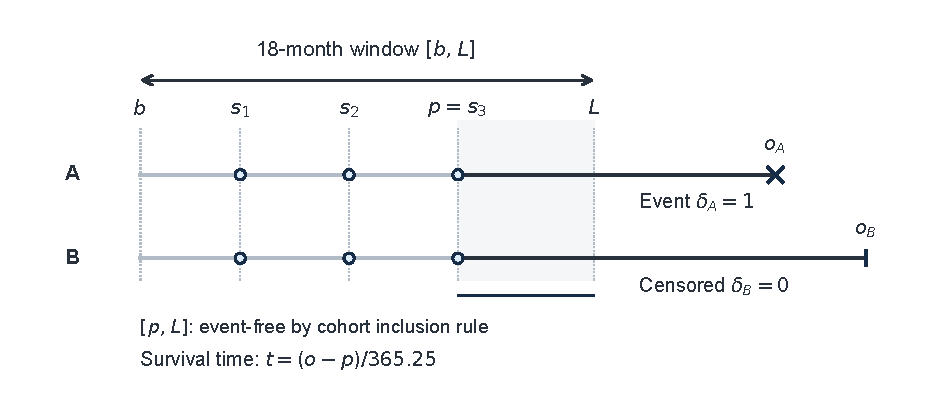
\includegraphics[width=\textwidth]{image_en/concept-survival.pdf}
\caption{Illustration of progression events and right-censoring in survival analysis}
\label{fig:concept-survival}
\end{figure}

The Cox proportional hazards model \cite{cox1972regression} expresses the instantaneous event rate (hazard function) $h_i(t)$ of individual $i$ at time $t$ as the product of two components:
\begin{equation}
 h_i(t)=h_0(t)\exp(\eta_i).
 \label{eq:cox-hazard}
\end{equation}
Here, $h_0(t)$ denotes the population-level \emph{baseline hazard function} over time, while $\eta_i = f_\theta(x_i)$ represents the individual \emph{log-risk score} estimated from input features $x_i$ via a deep neural network parameterized by $\theta$ (following the paradigm of DeepSurv \cite{katzman2018deepsurv}). A key advantage of the Cox formulation is that the hazard ratio between any two individuals $i$ and $j$ equals $\exp(\eta_i - \eta_j)$, which is entirely independent of time $t$. This implies that an individual assigned a higher log-risk score $\eta$ exhibits a higher instantaneous risk of progression at every point across the follow-up horizon.

By virtue of this time-invariance property, training the neural network does not require estimating the nonparametric baseline hazard $h_0(t)$; instead, one directly minimizes the negative Cox partial log-likelihood \cite{cox1972regression,katzman2018deepsurv}:
\begin{equation}
 \mathcal L_{\rm Cox}=-\sum_{i:\delta_i=1}\left[\eta_i-\log\sum_{j\in\mathcal R(t_i)}\exp(\eta_j)\right],
 \label{eq:cox-loss}
\end{equation}
where $\mathcal R(t_i)=\{j:t_j\geq t_i\}$ denotes the \emph{risk set} comprising all individuals who remain under active follow-up and have not experienced an event just prior to time $t_i$. Intuitively, this loss function compels the model to assign a higher risk score $\eta_i$ to the individual experiencing an event at $t_i$ than the scores $\eta_j$ of all individuals remaining event-free in the risk set at that moment; meanwhile, right-censored participants still contribute appropriately to the normalizing denominator $\mathcal R(t_i)$ up until the time they leave the study. When multiple events occur at tied survival times, I employ Breslow's approximation so that tied events share a common risk-set denominator consistently \cite{breslow1974covariance}. To evaluate the model's global ranking capability, the standard metric is Harrell's concordance index (C-index)---representing the proportion of comparable patient pairs in which the individual who experiences the event earlier is correctly assigned a higher risk score \cite{harrell1996multivariable}.

In longitudinal data analysis, a closely related methodological concept is \emph{landmarking}: at a pre-specified landmark time point, the prognostic model utilizes only information collected up to that landmark to predict future outcomes among individuals who remain event-free in the risk set \cite{vanhouwelingen2007dynamic}. The exact definition of the observation window and cohort eligibility milestone used in this thesis is detailed in Chapter~\ref{chap:method}.

\subsection{Time-Aware LSTM (T-LSTM) and Additive Attention}
\label{sec:background-temporal}
Long Short-Term Memory (LSTM) networks process sequential data effectively by maintaining and updating an internal memory state across successive steps \cite{hochreiter1997lstm}. However, standard LSTM architectures implicitly assume that the elapsed time between any two consecutive sequence steps is uniform. In real-world clinical records, the time gap between two consecutive visits varies substantially: it might be 3 months for one patient but up to 12 months for another. Clearly, clinical observations recorded 12 months ago generally carry less immediate relevance to the current state than observations acquired just 3 months prior \cite{baytas2017patient}.

The Time-Aware LSTM (T-LSTM) architecture proposed by Baytas et al. \cite{baytas2017patient} overcomes this limitation by incorporating the actual elapsed time interval $\Delta t$ between consecutive visits directly into the memory update equations: the previous cell memory $c_{t-1}$ is decomposed into a long-term component (preserved intact) and a short-term component (discounted monotonically as a decreasing function of $\Delta t$) before being combined with the new information from the current visit.

Once the T-LSTM generates the sequence of hidden states $h_t$ corresponding to each clinical visit, rather than passively relying only on the final hidden state, the model employs an additive attention mechanism to adaptively aggregate all visits using data-driven weights. The concept of weighted sequence aggregation originates from Bahdanau et al. \cite{bahdanau2015attention}; in this thesis, I implement scoring via a learnable context vector $\bm v$ following Yang et al. \cite{yang2016hierarchical}:
\begin{equation}
 e_t=\bm v^\top\tanh(W_hh_t+b_h),\qquad
 \alpha_t=\frac{\exp(e_t)}{\sum_k\exp(e_k)},\qquad
 z=\sum_t\alpha_th_t.
 \label{eq:additive-attention}
\end{equation}
Here, the attention weight $\alpha_t \in (0,1)$ quantifies the relative informational contribution of visit $t$, and $z$ serves as the unified longitudinal representation summarizing the patient's entire visit history. Figure~\ref{fig:concept-longitudinal} illustrates the synergistic integration of T-LSTM and additive attention across a three-visit sequence.

\begin{figure}[H]
\centering
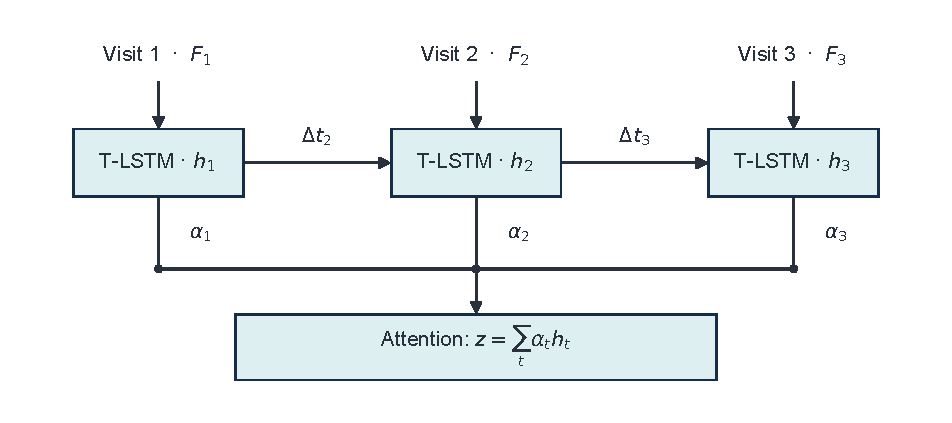
\includegraphics[width=\textwidth]{image_en/concept-longitudinal.pdf}
\caption{Principle of aggregating irregularly spaced longitudinal visit sequences via T-LSTM and additive attention}
\label{fig:concept-longitudinal}
\end{figure}

\section{The Three Information Sources and Feature Representations}
This thesis integrates three standard and widely adopted data modalities in Alzheimer's disease research: 3D structural MRI scans, whole-brain radiomics features, and clinical assessment scores. Table~\ref{tab:background-inputs} and Figure~\ref{fig:concept-sources} summarize the informational nature and specific technical considerations of each modality.

\begin{table}[H]
\centering\small
\caption[The three information sources in the prognostic task]{Informational nature and technical considerations of the three input modalities.}
\label{tab:background-inputs}
\begin{tabularx}{\linewidth}{@{}L{2.5cm}Y Y@{}}
\toprule
\textbf{Modality} & \textbf{Primary Information} & \textbf{Key Technical Consideration} \\
\midrule
3D structural MRI & Brain anatomical morphology; automated representation learning via 3D CNN & Requires standardizing head pose, voxel grid dimensions, and intensity scale without distorting anatomical geometry \\
Radiomics & Quantitative mathematical descriptors of shape, intensity distribution, and tissue texture & Texture feature values depend on the gray-level discretization scheme \cite{zwanenburg2020ibsi} \\
Clinical scores & Cognitive test (MMSE) and functional rating (CDR) scores & Directly tied to the outcome event definition; requires strict separation between input and outcome windows \\
\bottomrule
\end{tabularx}
\end{table}

\begin{figure}[H]
\centering
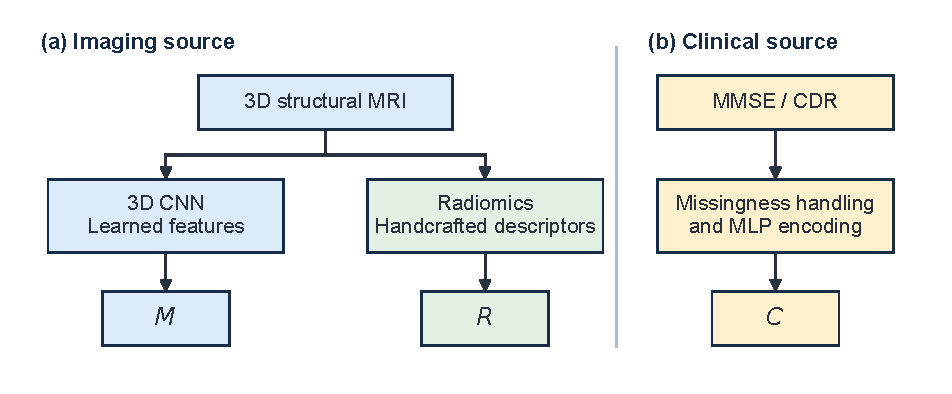
\includegraphics[width=\textwidth]{image_en/concept-sources.pdf}
\caption{Provenance and relationships among the three data representation streams at each visit}
\label{fig:concept-sources}
\end{figure}

More specifically, each information source fulfills a specialized representational role:
\begin{enumerate}
\item \emph{3D structural MRI}: visually captures brain anatomical morphology at the time of scanning \cite{jack2008adnimri}. In medical deep learning, 3D residual convolutional architectures such as ResNet \cite{he2016deep}, particularly when initialized with weights pretrained on diverse 3D medical imaging datasets such as MedicalNet \cite{chen2019med3d}, are widely favored for learning representations directly from the whole-brain volume---rather than cropping only the local hippocampal region as in several earlier studies \cite{li2019hippocampal}.
\item \emph{Radiomics features}: represent explicitly defined mathematical descriptors designed to quantify spatial geometry, first-order voxel intensity statistics, and spatial texture patterns within the brain mask (such as contrast derived from the Gray-Level Co-occurrence Matrix, GLCM). These feature definitions have been rigorously standardized by the IBSI community \cite{zwanenburg2020ibsi} and implemented in the PyRadiomics library \cite{vangriethuysen2017computational}. Because radiomics feature sets are typically high-dimensional and exhibit strong internal collinearity, Principal Component Analysis (PCA) \cite{jolliffe2016pca} serves as an effective dimensionality reduction tool prior to neural network encoding.
\item \emph{Clinical data}: the MMSE scale \cite{folstein1975mmse} evaluates global cognitive function, whereas the CDR scale \cite{morris1993cdr} assesses both cognitive performance and functional independence in daily life. Scores collected during the input observation window provide direct signals regarding the patient's current clinical state, kept strictly separate from post-milestone assessments used to determine progression outcomes.
\end{enumerate}

\section{Multimodal Fusion and Interaction Parameterization}
\label{sec:background-fusion}
Once each data modality has been mapped into a feature vector, the next central challenge is fusing them into a joint representational space \cite{baltrusaitis2019multimodal}. The most direct and common strategy is \emph{concatenation}: stacking the constituent vectors end to end to form a longer vector. While concatenation introduces no extra parameters at the combination step, its inherent limitation is that it fails to explicitly construct second-order cross-modal terms; consequently, discovering complex nonlinear relationships across modalities is left entirely to subsequent hidden layers.

In contrast, the \emph{outer product} multiplies every coordinate of the first modality by every coordinate of the second modality, explicitly constructing all second-order bilinear pairwise interactions \cite{zadeh2017tensor}. Figure~\ref{fig:concept-fusion} illustrates this fundamental distinction on two 2-dimensional vectors: concatenation yields a 4-element vector of independent coordinates, whereas the outer product forms a $2\times2$ matrix containing all four cross-products $x_i y_j$.

\begin{figure}[H]
\centering
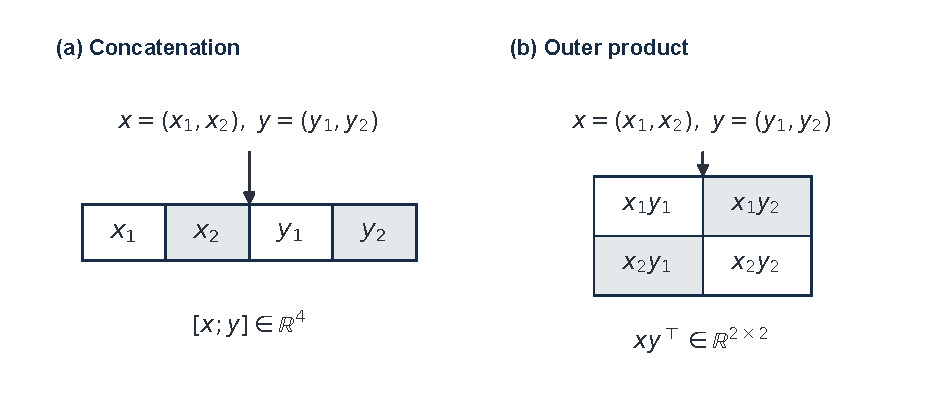
\includegraphics[width=\textwidth]{image_en/concept-fusion.pdf}
\caption{Comparison between feature concatenation and outer-product interaction on a two-dimensional example}
\label{fig:concept-fusion}
\end{figure}

\subsection{From Outer Products to Low-Rank CP Tensor Decomposition}
The primary obstacle to deploying full outer products in neural architectures is computational parameter explosion. Consider two arbitrary feature vectors $x\in\mathbb R^{d_x}$ and $y\in\mathbb R^{d_y}$. If the outer-product matrix $xy^\top \in \mathbb R^{d_x\times d_y}$ is flattened and projected through a standard linear layer into a $d_o$-dimensional output space, each output coordinate $h_k$ ($k=1,\dots,d_o$) is computed as a weighted combination of all cross-products:
\begin{equation}
 h_k=\sum_{i=1}^{d_x}\sum_{j=1}^{d_y}\mathcal W_{kij}x_i y_j+b_k,
 \label{eq:full-bilinear}
\end{equation}
where $\mathcal W\in\mathbb R^{d_o\times d_x\times d_y}$ acts as a third-order weight tensor. Under this formulation, the number of learnable weights reaches $d_o d_x d_y$ (excluding the bias vector $b$). For the actual dimensions used in this thesis ($d_x=32$, $d_y=32$, and $d_o=128$), a single bilinear interaction layer alone requires $32 \times 32 \times 128 = 131\,072$ weights---an excessively large capacity relative to a training cohort of a few hundred patients, placing the model at high risk of overfitting \cite{liu2018lowrank}.

To eliminate this parameter bottleneck while retaining the capacity to capture bilinear interactions, \emph{Canonical Polyadic (CP) tensor decomposition} \cite{carroll1970candecomp,kolda2009tensor} approximates the third-order weight tensor $\mathcal W$ as a sum of $Q$ rank-one tensors, where $Q$ is a small positive integer termed the \emph{decomposition rank}:
\begin{equation}
 \mathcal W_{kij}\approx\sum_{q=1}^Q O_{kq}A_{iq}B_{jq}.
 \label{eq:cp-concept-math}
\end{equation}
Substituting Eq.~(\ref{eq:cp-concept-math}) into Eq.~(\ref{eq:full-bilinear}) and rearranging the summation order reduces the cumbersome three-way tensor projection into a sequence of three lightweight operations:
\begin{equation}
 h=O\bigl[(A^\top x)\odot(B^\top y)\bigr]+b,
 \label{eq:cp-hadamard}
\end{equation}
where $A\in\mathbb R^{d_x\times Q}$, $B\in\mathbb R^{d_y\times Q}$, and $O\in\mathbb R^{d_o\times Q}$ are three low-rank factor matrices optimized directly via backpropagation, and $\odot$ denotes the element-wise Hadamard product. Rather than multiplying all coordinate pairs in the original space before compressing, the CP factorization projects $x$ and $y$ into a shared $Q$-dimensional latent space first, computes element-wise products within this low-rank space, and then projects the result linearly to the $d_o$-dimensional output space (Figure~\ref{fig:cp-intro}). Returning to the example with $d_x=32, d_y=32, d_o=128$: choosing rank $Q=8$ reduces the learnable weight count dramatically from $131\,072$ down to $Q(d_x + d_y + d_o) = 8 \times (32+32+128) = 1\,536$ (a reduction of nearly 99\%). This low-rank parameterization principle also forms the core foundation of prominent multimodal fusion architectures such as LMF \cite{liu2018lowrank} and MUTAN \cite{benyounes2017mutan}.

\begin{figure}[H]
\centering
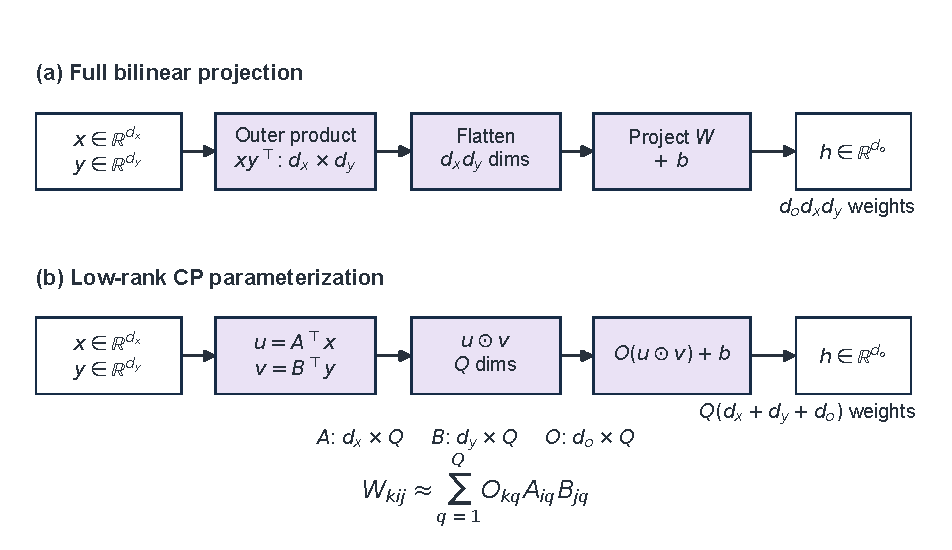
\includegraphics[width=\textwidth]{image_en/cp-concept-general.pdf}
\caption{Comparison between full bilinear projection and low-rank CP parameterization}
\label{fig:cp-intro}
\end{figure}

\subsection{Principle of Gated Residual Connections}
Once a bilinear interaction representation between two sources has been computed, completely replacing each modality's original representation with the interaction vector risks losing modality-specific signals, especially when one of the two sources suffers from measurement noise. To address this vulnerability, an effective principle in multimodal fusion is \emph{gated residual fusion}: preserving the direct pathway of the original representation and adding the interaction component only after modulating it through an input-dependent adaptive gate.

This principle has demonstrated effectiveness across diverse application domains; two recent arXiv preprints in multimodal video analysis illustrate representative variants:
\begin{enumerate}
\item \emph{Text Residual Fusion} by Ryumina et al. (2026) \cite{ryumina2026residual}: utilizes the text representation as the primary backbone stream, while audio, facial, and contextual streams contribute residual updates through input-dependent gates prior to layer normalization (Figure~\ref{fig:literature-gates}(a)).
\item \emph{DyFADet+} by Liu et al. (2026) \cite{liu2026motion}: treats the RGB visual stream as the main transmission pathway, while skeleton motion features pass through a gating unit scaled by a fixed constant $\alpha=0.5$ before residual addition (Figure~\ref{fig:literature-gates}(b)).
\end{enumerate}

\begin{figure}[H]
\centering
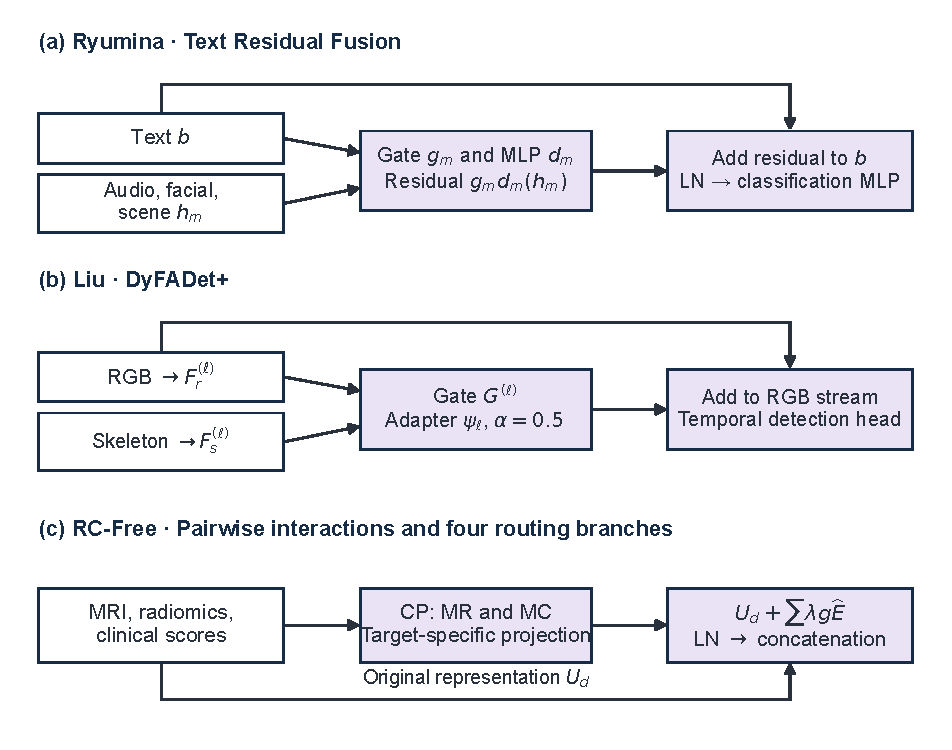
\includegraphics[width=\textwidth]{image_en/literature-gates.pdf}
\caption[Gated residual fusion mechanisms]{Illustration of gated residual connection principles synthesized by the author: (a) following Ryumina et al.~\cite{ryumina2026residual}, (b) following Liu et al.~\cite{liu2026motion}, and (c) the modality-specific gated residual routing scheme adopted in this thesis.}
\label{fig:literature-gates}
\end{figure}

Unlike the two aforementioned designs that anchor residual updates onto a single dominant stream, in the architecture proposed in this thesis, every input modality preserves its own dedicated representation pathway and receives pairwise interaction residuals through independent dynamic gates paired with learnable scaling coefficients (schematically illustrated in Figure~\ref{fig:literature-gates}(c)). The mathematical formulation and detailed architectural structure of this mechanism are presented in Section~\ref{sec:gated-routing} of Chapter~\ref{chap:method}.

\section{Related Work and Research Gaps}
\label{sec:related-work}
In recent years, numerous machine learning and deep learning methodologies have been proposed to tackle the problem of predicting MCI-to-dementia progression. Table~\ref{tab:related} systematizes four representative research directions in the literature and highlights the specific elements inherited by this thesis.

\begin{table}[H]
\centering\small
\renewcommand{\arraystretch}{1.02}
\caption[Summary of related work]{Major research directions, representative studies, and connections to this thesis.}
\label{tab:related}
\begin{tabularx}{\linewidth}{@{}L{2.8cm}Y Y@{}}
\toprule
\textbf{Approach} & \textbf{Representative Studies and Methods} & \textbf{Connection to This Thesis} \\
\midrule
Single-timepoint MRI & Li: hippocampal patches; Nakagawa: gray-matter volumes and deep survival network \cite{li2019hippocampal,nakagawa2020survival} & MRI representation learning within a survival analysis formulation \\
Longitudinal data & Li \& Fan: baseline MRI and longitudinal cognition \cite{li2019early}; Ding: cognitive and MRI sequences \cite{ding2023progression}; Dong: atrophy from longitudinal MRI pairs \cite{dong2021deepatrophy} & Exploiting temporal change dynamics for clinical prognosis \\
Radiomics and clinical scores & Tang et al.: LASSO--Cox combining radiomics, clinical scores, and laboratory markers \cite{tang2021individualized} & Motivation for verifying the complementary value of radiomics and clinical features \\
Longitudinal deep MRI survival & Aghajanian et al.: CNN--PCA--T-LSTM, attention, and Cox partial log-likelihood loss \cite{aghajanian2025longitudinal} & Direct reference pipeline, event definition, and risk stratification framework \\
\bottomrule
\end{tabularx}
\end{table}

Among these works, the study by Aghajanian et al. \cite{aghajanian2025longitudinal} serves as the most direct reference point. The authors selected 228 participants with MCI from ADNI who had at least three T1-weighted MRI scans within the first 18 months, employed a CNN to extract per-scan features, compressed them via PCA fitted on the training set (retaining 99\% explained variance), and trained a T-LSTM network (with an attention ablation) under the Cox loss. Crucially, when they experimented with concatenating gray-matter radiomics features into the T-LSTM with attention model, the discriminatory C-index decreased slightly rather than improving, leading the authors to retain only CNN-derived MRI features in their final model \cite{aghajanian2025longitudinal}.

\subsection{Research Gaps}
\label{sec:research-gaps}
It is important to emphasize that the negative conclusion regarding radiomics in Aghajanian et al. is tied to simple feature concatenation and a decoupled two-stage extraction pipeline. That result leaves open the question of whether explicitly modeling bilinear cross-modal interactions among MRI, radiomics, and clinical scores within a unified end-to-end deep learning architecture can unlock the prognostic potential of these complementary modalities. Motivated by this key research gap, I propose and empirically verify two architectural designs within a unified end-to-end training pipeline:
\begin{enumerate}[itemsep=0.1em,topsep=0.2em]
\item \emph{Parameterizing pairwise interactions via CP tensor decomposition}: replacing full bilinear projection layers with rank-$Q$ CP factorization to capture second-order cross-modal interactions while strictly controlling parameter complexity.
\item \emph{Pruning redundant direct interactions (RC-Free)}: retaining all three input modalities while activating only the two MRI-centered interaction pairs (MR and MC) and omitting the direct RC pair, then benchmarking this design systematically against all alternative pairwise topologies in Chapter~\ref{chap:results}.
\end{enumerate}
